\section{Simulación}
A partir de los componentes seleccionados, se simula el circuito con \textit{LTSpice}.

Para que la simulación se asemeje lo más posible al circuito realizable, se seleccionarán capacitores de valores normalizados lo más cercano posible a los calculados, es decir

\[
\begin{array}{|c|c|c|}
\hline
\textbf{Parameter} & \textbf{Value (F)} & \textbf{Valor comercial} \\
\hline
C_1 & 94.451E-12 & 100 \, \text{pF} \\
C_2 & 364.183E-12 & 330 \, \text{pF} \\
C_3 & 752.132E-12 & 680 \, \text{pF} \\
C_4 & 83.307E-12 & 82 \, \text{pF} \\
\hline
\end{array}
\]

\subsection{Respuesta en Frecuencia}

Se mide la salida sin $R_L$ para disminuir el ancho de banda, obteniendo $f_0 = 17.82 MHz$ a partir del cursor.

\begin{figure}[H]
    \centering
    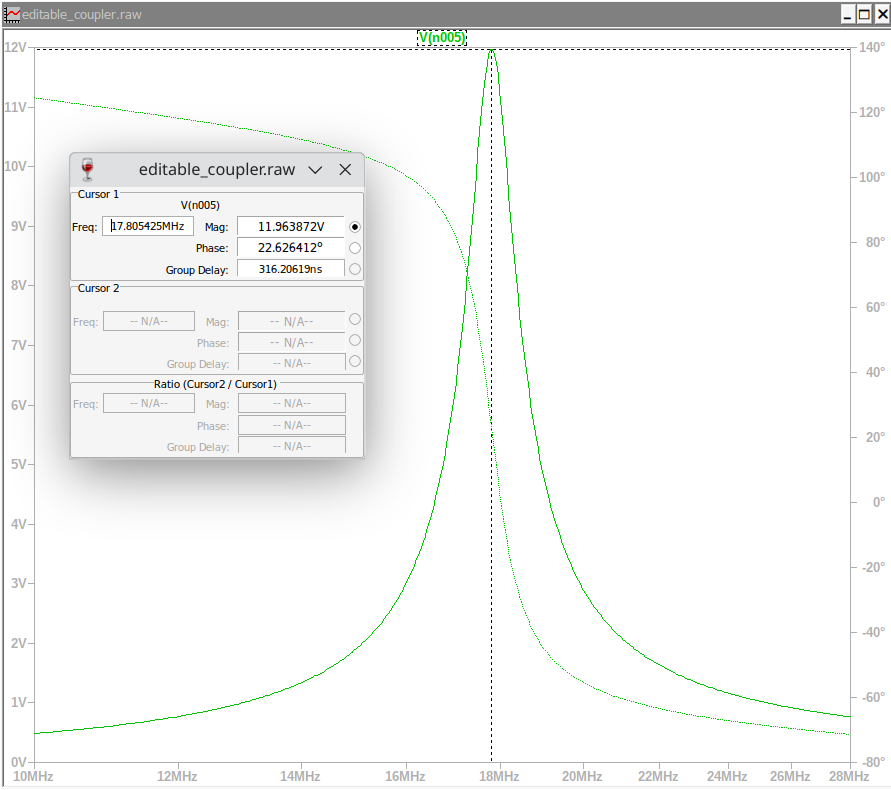
\includegraphics[width=0.5\linewidth]{fig/bode.png}
    \caption{respuesta en frecuencia del acoplador simulado}
    \label{fig:enter-label}
\end{figure}

\subsection{Impedancia de Entrada y Salida}

La impedancia de entrada está dada por la diferencia entre la caida de tensión en la entrada del circuito con y sin el acoplador conectado.

\begin{figure}[H]
    \centering
    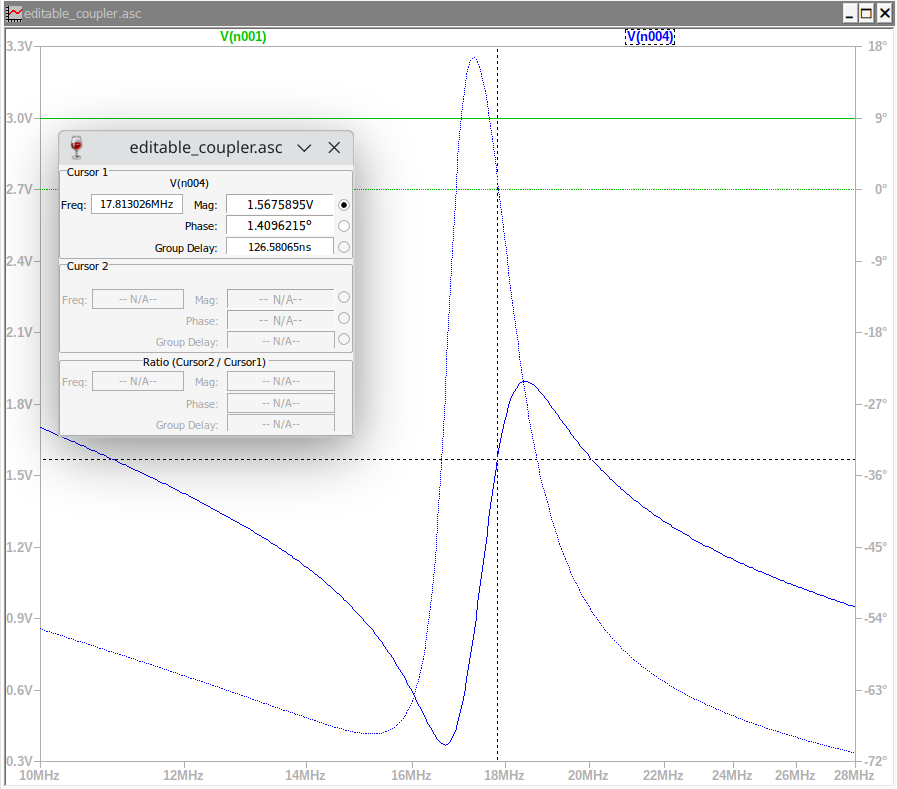
\includegraphics[width=0.5\linewidth]{fig/zin.png}
    \caption{medición de la impedancia de entrada}
    \label{fig:enter-label}
\end{figure}

Se observa que la tensión en la entrada cae a aproximadamente la mitad al conectar el acoplador para la frecuencia de resonancia, lo cual indica una impedancia correctamente adaptada. Matemáticamente, esto es

$$
Z_{in} = \frac{R_a}{Vg/Vi-1} = \frac{50\Omega}{3V/1.56-1} = 54.16\Omega
$$

La impedancia de salida se puede medir al contrastar la caída de tensión sobre la salida del acoplador al conectar y desconectar la carga.

\begin{figure}[H]
    \centering
    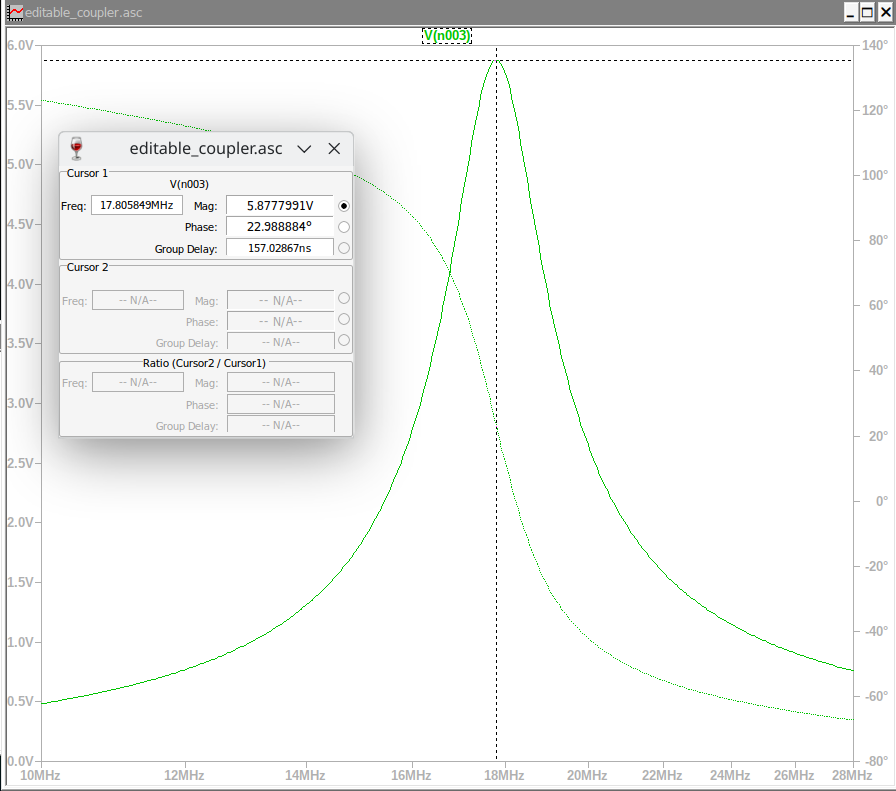
\includegraphics[width=0.5\linewidth]{fig/zo2.png}
    \caption{medición de la tensión de salida con carga}
    \label{fig:enter-label}
\end{figure}

\begin{figure}[H]
    \centering
    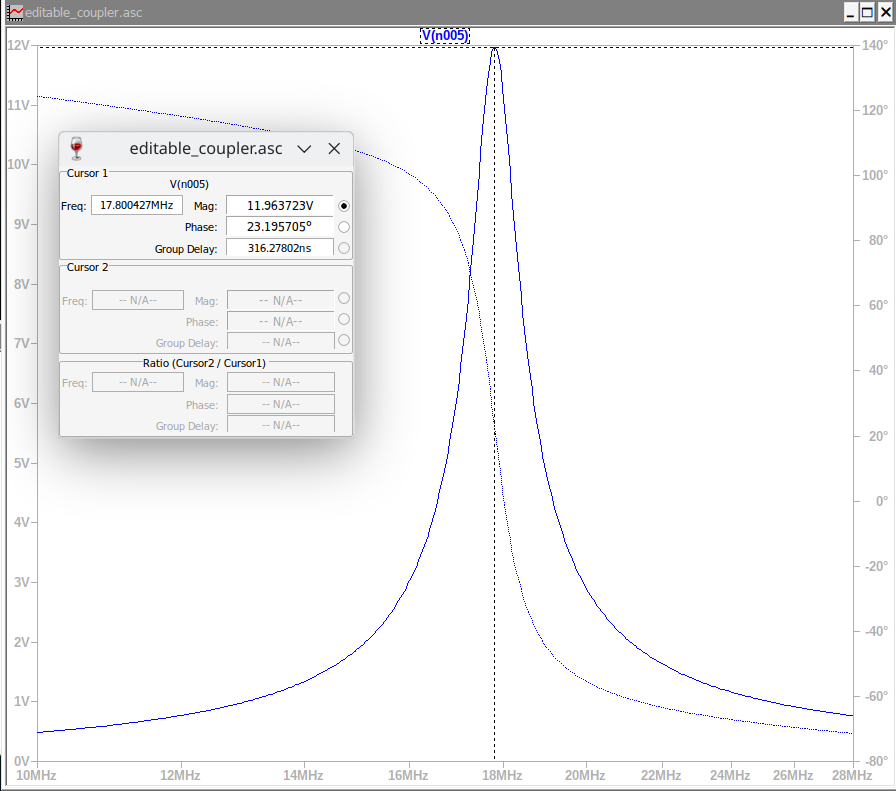
\includegraphics[width=0.5\linewidth]{fig/zout.png}
    \caption{medición de la tensión de salida sin carga}
    \label{fig:enter-label}
\end{figure}


$$
Z_{out} = R_L(\frac{V_O}{V_L}-1)= 1K\Omega(\frac{11.96V}{5.8V}-1)=1.02K\Omega
$$

\subsection{Ancho de Banda}
A partir de los 3db de atenuación en la carga del acoplador, se tiene

\begin{figure}[H]
    \centering
    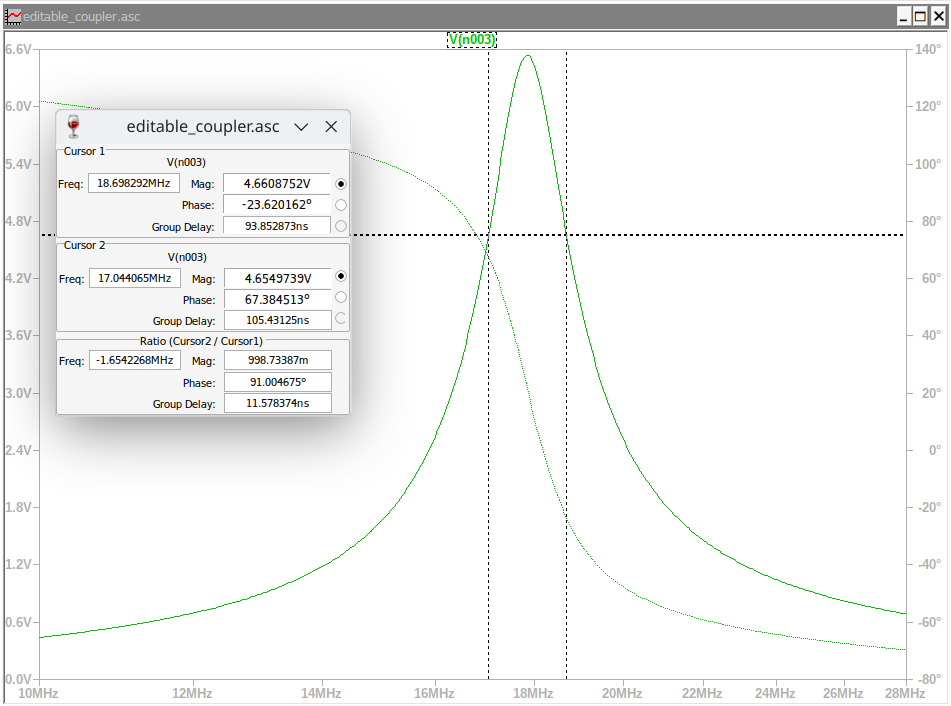
\includegraphics[width=0.5\linewidth]{fig/bws.png}
    \caption{ancho de banda en simulador}
    \label{fig:enter-label}
\end{figure}

$$
BW = 18.76MHz - 16.90MHz = 1.65MHz
$$



